\setcounter{step}{0}
%------------------------------------------
% information doc
\subsection{Florentins au chocolat}
%------------------------------------------

\begin{ingredient}

%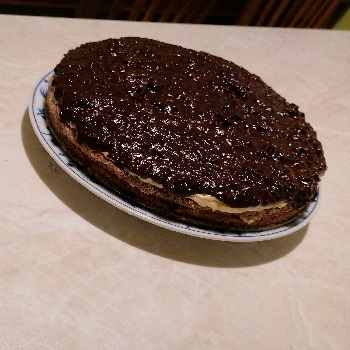
\includegraphics[height=5.5cm]{images/daim}
\def\portions{4}%
\textbf{{\normalsize Ingrediencie (\portions porcie):}}

%\vspace{0.5cm}
\begin{main}
	\item 4 cà.S de sucre en poudre
	\item 1 cà.S de crème liquide
	\item 1 cà.S de miel
	\item 1 grosse noix de beurre
	\item 35 gr d’amandes effilées
	\item 50 gr de chocolat au lait ou chocolat blanc
\end{main}
\begin{subingredient}{Test subingredient}
	\item 1 cà.c de test1
	\item 1 à 2 cà.S de test2
	\item 3 gouttes de test3
	\item 8 morceaux de test4.	
\end{subingredient}

\end{ingredient}
\begin{recipe}
\textbf{{\normalsize Príprava:}}
\begin{enumerate}
\item{Préchauffez votre four à 180°C (th.6).}
\item{Dans une casserole, faites bouillir le sucre en poudre avec la crème liquide, le beurre et le miel.}
\item{Une fois que le sucre prend une jolie coloration brune, versez les amandes effilées dans la casserole, et remuez bien pour napper l’intégralité des amandes.}	
\item{Pour la cuisson au four vous avez 2 possibilités : Soit vous versez la « pâte » dans le fond de moules en silicone, type moules à muffins ou moules à tartelettes, soit vous étalez bien la « pâte », et rapidement car le caramel durcit vite, sur la plaque de votre four recouverte d’une feuille de papier sulfurisé, et après la cuisson vous découperez des cercles à l’aide d’un emporte-pièces rond.}
\item{Dans tous les cas, mettez la « pâte » au four pendant 3 à 5 minutes. A la sortie du four, soit vous découpez tout de suite des ronds à l’aide de l’emporte-pièces, soit vous laissez refroidir les florentins avant de les démouler de vos moules à muffins.}
\item{Pendant que les florentins refroidissent, faites fondre le chocolat au lait ou blanc soit au bain-marie, soit au micro-ondes à faible puissance, soit dans une petite casserole à feu doux.}
\item{Trempez ensuite la moitié des florentins dans le chocolat fondu et mettez-les au réfrigérateur pendant une bonne vingtaine de minutes pour que le chocolat prenne bien.}
\item{Test substep}:
\begin{enumerate}
\item{Blabla}
\item{Blabla}
\end{enumerate}

\end{enumerate}

\end{recipe}

\begin{notes}

\end{notes}	
\clearpage